\documentclass[12pt]{article}
\usepackage{amsmath,amsthm,amsfonts,amscd,amssymb,mathrsfs,cite}
\usepackage{tikz}
\usepackage{pgfplots}
\usepackage[utf8]{inputenc}
\usetikzlibrary{patterns}
\tikzset{dottednode/.style={
        dash pattern=on 1.5pt off 4pt, 
        line width=1.9pt
}}
\tikzset{dashednode/.style={dash pattern=on 6pt off 5pt}}
\usepackage{color}

\begin{document}

    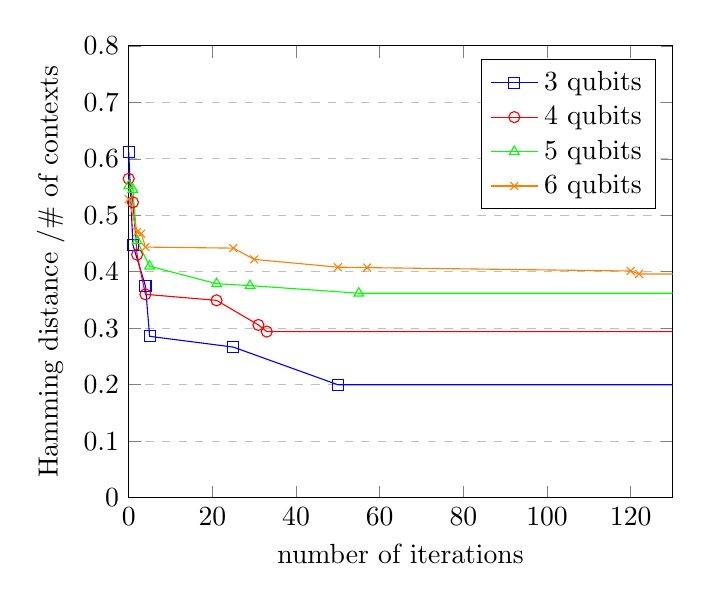
\begin{tikzpicture}
    \begin{axis}[
        xlabel={number of iterations}, ylabel={Hamming distance /\# of contexts},
        xmin=0, xmax=130,
        ymin=0, ymax=0.8,
        xtick={0,20,...,130},
        ytick={0,0.1,...,1},
        legend pos=north east,
        ymajorgrids=true,
        grid style=dashed,
        width=0.7\textwidth,
    ]

    \addplot[
        color=blue,
        mark=square,
        y filter/.expression={y/315},
        ]
        coordinates {
        (0,193) (1,141) (4,118) (5,90) (25,84) (50,63)      (1000,63)
        };
        \legend{$3$ qubits}


    \addplot[
        color=red,
        mark=o,
        y filter/.expression={y/5355},
        ]
        coordinates {
        (0,3024) (1,2800) (2,2304) (4,1928) (21,1871) (31,1638) (33,1575)      (1000,1575)
        };
        \addlegendentry{$4$ qubits}

    \addplot[
        color=green,
        mark=triangle,
        y filter/.expression={y/86955},
        ]
        coordinates {
        (0,48032) (1,47449) (2,39532) (5,35636) (21,32944) (29,32650) (55,31479)      (1000,31479)
        };
        \addlegendentry{$5$ qubits}

    \addplot[
        color=orange,
        mark=x,
        y filter/.expression={y/1396395},
        ]
        coordinates {
        (0,738219) (2,656892) (3,652791) (4,619539) (25,616998) (30,589224) (50,569892) (57,568824) (120,560384) (122,553140)     (1000,553140)

        };
        \addlegendentry{$6$ qubits}

    \end{axis}
    \end{tikzpicture}

\end{document}